\chapter{System Architecture}

\section{System Context}

\begin{figure}[H]
\centering
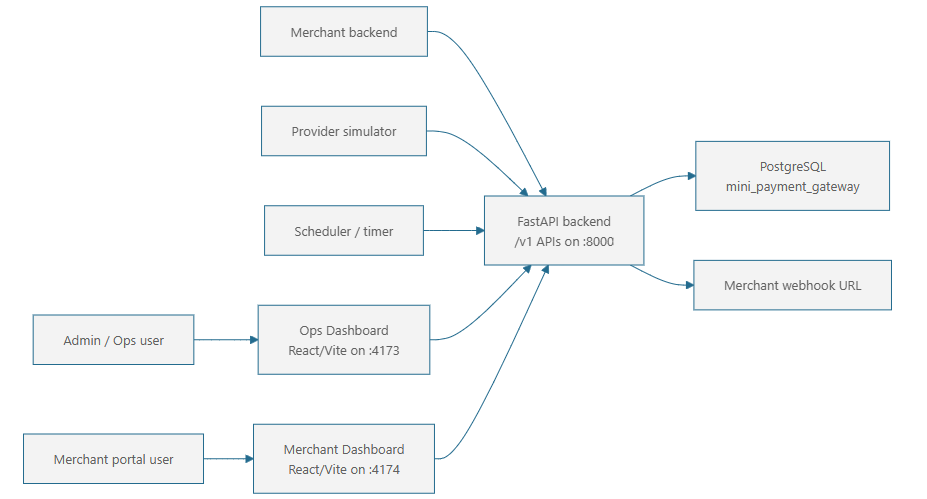
\includegraphics[width=\linewidth]{figures/system-context-diagram.png}
\caption{System context diagram for the implemented Mini Payment Gateway.}
\end{figure}

The implemented system consists of four main runtime components: a FastAPI
backend, PostgreSQL, the internal Ops Dashboard, and the Merchant Dashboard.
The dashboards are not presentation-only shells. Each depends on dedicated API
surfaces, access boundaries, and data representations that match its actor.

\section{Runtime Topology}

\begin{table}[H]
\centering
\caption{Runtime components and responsibilities}
\begin{tabularx}{\textwidth}{L{0.22\textwidth}L{0.24\textwidth}Y}
\toprule
\textbf{Component} & \textbf{Runtime shape} & \textbf{Responsibility} \\
\midrule
FastAPI backend & Application service & Exposes merchant APIs, provider callbacks, internal Ops APIs, internal auth, merchant portal auth, analytics, and recovery endpoints. \\
PostgreSQL & Persistent database & Stores merchant, transaction, refund, webhook, callback, reconciliation, audit, internal user, and merchant user data. \\
Ops Dashboard & Separate frontend application & Supports internal monitoring, merchant operations, user administration, and evidence review. \\
Merchant Dashboard & Separate frontend application & Supports merchant-scoped overview, analytics, explorers, profile, credentials, and password change. \\
\bottomrule
\end{tabularx}
\end{table}

\section{Authentication, Authorization, And Trust Boundaries}

\begin{table}[H]
\centering
\caption{Actor and authentication matrix}
\begin{tabularx}{\textwidth}{L{0.20\textwidth}L{0.21\textwidth}L{0.24\textwidth}Y}
\toprule
\textbf{Actor} & \textbf{API surface} & \textbf{Authentication} & \textbf{Scope source} \\
\midrule
Merchant backend & Merchant API & HMAC headers & Authenticated merchant credential. \\
Admin/Ops user & Ops API & Internal HttpOnly session cookie & Internal user role \texttt{ADMIN} or \texttt{OPS}. \\
Admin user & Ops portal-user API & Internal HttpOnly session cookie & Internal \texttt{ADMIN} role. \\
Merchant portal user & Merchant Portal API & Merchant HttpOnly session cookie & \texttt{merchant\_users.merchant\_db\_id}. \\
Provider simulator & Provider callback API & Environment-local simulator trust in MVP & Callback payload references existing payment or refund rows. \\
\bottomrule
\end{tabularx}
\end{table}

\begin{figure}[H]
\centering
\begin{tikzpicture}[node distance=14mm and 18mm]
  \node[actor] (merchantBackend) {Merchant backend};
  \node[actor, below=of merchantBackend] (opsUser) {Admin / Ops};
  \node[actor, below=of opsUser] (portalUser) {Merchant portal user};
  \node[box, right=34mm of opsUser, text width=33mm] (api) {FastAPI backend};
  \node[db, right=of api] (db) {PostgreSQL};

  \node[boundary, fit=(merchantBackend), label=above:{Merchant integration boundary}] {};
  \node[boundary, fit=(opsUser), label=above:{Internal operations boundary}] {};
  \node[boundary, fit=(portalUser), label=below:{Merchant portal boundary}] {};

  \draw[autharrow] (merchantBackend) -- node[above,sloped,font=\scriptsize,fill=white,inner sep=1pt]{HMAC headers} (api);
  \draw[autharrow] (opsUser) -- node[above,sloped,font=\scriptsize,fill=white,inner sep=1pt]{internal session cookie} (api);
  \draw[autharrow] (portalUser) -- node[below,sloped,font=\scriptsize,fill=white,inner sep=1pt]{merchant session cookie} (api);
  \draw[arrow] (api) -- (db);
\end{tikzpicture}
\caption{Trust boundaries and authentication mechanisms. Merchant API
credentials are not reused for dashboard login.}
\end{figure}

This separation is one of the project's core architectural decisions. Merchant
Portal APIs never accept a client-supplied \texttt{merchant\_id} after login.
The backend derives scope from the authenticated merchant portal user to prevent
cross-merchant reads.

\section{Key Request Flows}

The report focuses on three flows that illustrate the main design decisions:

\begin{enumerate}
  \item \textbf{Merchant creates a payment}: merchant backend sends
  \apiendpoint{POST}{/v1/payments}; backend verifies merchant readiness, creates
  or reuses a payment row, generates QR content, and returns the transaction.
  \item \textbf{Admin provisions merchant portal user}: Admin uses Ops Dashboard
  to call \apiendpoint{POST}{/v1/ops/merchants/\{merchant\_id\}/portal-users};
  backend requires an internal \texttt{ADMIN} session, stores a password hash,
  writes audit evidence, and returns a generated password once.
  \item \textbf{Merchant reads analytics}: Merchant Dashboard calls
  \apiendpoint{GET}{/v1/merchant-portal/analytics?days=30}; backend
  authenticates the merchant session, aggregates payment, refund, and webhook
  rows by day, returns zero-filled buckets, and never accepts a client-supplied
  merchant scope.
\end{enumerate}

\section{Operational And Deployment Overview}

The deployed sandbox uses a high-level split between verification and runtime
execution. GitHub-hosted checks validate backend and frontend changes, while a
self-hosted runner on the sandbox host executes the deploy job locally against a
persistent checkout and Docker Compose runtime.

This report intentionally keeps deployment discussion at architecture level
only. The operational runbooks, host facts, and recovery commands are maintained
in \code{docs/infrastructure/}, while the report captures only the reason the
topology exists: small-scope CI/CD, host-local runtime secrets, and a direct
mapping between the implemented codebase and the running sandbox environment.
